% Experiments

\subsection{Experimental Setup}

\paragraph{Model.}
We use a 1D Fourier Neural Operator with residual connections (FNO1d-Residual).
Table~\ref{tab:model-settings} summarizes the architecture and training configuration.
The model has approximately 93k parameters---deliberately kept small to establish a
meaningful baseline rather than optimize for peak performance.

\begin{table}[h]
\centering
\caption{Baseline FNO model and training settings.}
\label{tab:model-settings}
\begin{tabular}{ll}
\toprule
\textbf{Architecture} & \\
\midrule
Model & FNO1d-Residual \\
Fourier modes & 12 \\
Width (hidden dim) & 48 \\
Fourier layers & 3 \\
Activation & GELU \\
Dropout & 0.1 \\
Parameters & ${\sim}$93k \\
\midrule
\textbf{Training} & \\
\midrule
Optimizer & AdamW \\
Learning rate & $10^{-3}$ \\
LR scheduler & ReduceLROnPlateau (patience=10, factor=0.5) \\
Weight decay & $10^{-4}$ \\
Batch size & 32 \\
Max epochs & 150 \\
Early stopping & patience = 20 \\
\midrule
\textbf{Normalization} & \\
\midrule
Method & Per-channel mean/std (training set) \\
\bottomrule
\end{tabular}
\end{table}

\paragraph{Dataset protocol.}
For each of the five DDE families, we generate 8{,}000 training, 1{,}000 validation,
and 2{,}000 test samples.  The prediction horizon is $T = 15$ with 256 uniformly spaced
output grid points ($\Delta t \approx 0.06$).  History functions are sampled as random
Fourier series on $[-\tau_{\max}, 0]$ with $\tau_{\max} = 2$.

\paragraph{Evaluation metric.}
We report the relative $L^2$ error on the future region ($t > 0$):
\begin{equation}
  \text{Rel.\ } L^2 = \frac{\|\hat{y} - y\|_2}{\|y\|_2},
\end{equation}
computed per sample and summarized as median and 95th percentile (P95) over
the test set.  The median captures typical performance while P95 captures tail
behavior on difficult samples.

\paragraph{Out-of-distribution splits.}
Beyond the in-distribution (ID) test set, we evaluate on three OOD splits:
\begin{itemize}
  \item \textbf{OOD-delay}: delay values $\tau > 1.3$ (held out from training range $[0.1, 2.0]$),
  \item \textbf{OOD-history}: spline-interpolated history functions (vs.\ Fourier series in training),
  \item \textbf{OOD-horizon}: extended prediction horizon $T = 20$ (vs.\ $T = 15$ in training).
\end{itemize}

\paragraph{Baseline.}
As a lower bound, we compare against a \emph{naive persistence} predictor
$\hat{y}(t) = y(0)$ for all $t > 0$, which simply extends the last observed value
of the history function.

% ------------------------------------------------------------------
\subsection{In-Distribution Results}

Table~\ref{tab:id-results} reports the ID test performance across all five families.
The families exhibit a clear difficulty spectrum: distributed-delay families
(DistExp, DistUniform) are easiest, followed by the single-delay Hutchinson equation,
the 2D oscillatory Van der Pol system, and finally the two-delay Linear2 family.

\begin{table}[h]
\centering
\caption{In-distribution test performance (relative $L^2$ error).
Families are ordered by increasing difficulty.}
\label{tab:id-results}
\begin{tabular}{lccc}
\toprule
Family & Median & P90 & P95 \\
\midrule
DistExp        & 0.077 & 0.413 & 0.683 \\
DistUniform    & 0.089 & 0.335 & 0.406 \\
Hutchinson     & 0.121 & 0.403 & 0.552 \\
Van der Pol    & 0.296 & 0.703 & 0.897 \\
Linear2        & 0.612 & 1.151 & 1.532 \\
\bottomrule
\end{tabular}
\end{table}

The difficulty ranking reveals a pattern: distributed delays, which smooth the
dependence on past states via integration, are easier to learn than discrete delays.
Among discrete-delay families, multi-delay systems (Linear2, with two interacting
delays $\tau_1$ and $\tau_2$) pose the greatest challenge.  The Van der Pol system's
difficulty stems from its 2D oscillatory dynamics and nonlinear coupling.

Table~\ref{tab:baseline-comparison} compares the FNO against the naive persistence
baseline.  The FNO achieves 4.6--31.8$\times$ improvement in median error and up to
31.8$\times$ at P95, confirming that the model learns meaningful delay dynamics
rather than trivially extrapolating the initial condition.

\begin{table}[h]
\centering
\caption{FNO vs.\ naive persistence baseline (relative $L^2$ error).}
\label{tab:baseline-comparison}
\begin{tabular}{lcccc}
\toprule
Family & Naive (Med.) & FNO (Med.) & Improv. & P95 Improv. \\
\midrule
Hutchinson  & 1.164 & 0.121 & 9.6$\times$  & 7.1$\times$ \\
Linear2     & 6.076 & 0.612 & 9.9$\times$  & 31.8$\times$ \\
Van der Pol & 1.352 & 0.296 & 4.6$\times$  & 2.6$\times$ \\
DistUniform & 0.707 & 0.089 & 8.0$\times$  & 4.5$\times$ \\
DistExp     & 0.567 & 0.077 & 7.4$\times$  & 2.9$\times$ \\
\bottomrule
\end{tabular}
\end{table}

Figure~\ref{fig:predictions} shows representative predictions for the easiest
(Hutchinson) and hardest (Linear2) families.  For Hutchinson, the FNO closely tracks
the reference solution including oscillatory behavior.  For Linear2, the model captures
the qualitative shape but accumulates error over time, particularly for samples with
large delay values.

\begin{figure}[h]
\centering
\begin{subfigure}[b]{0.48\textwidth}
  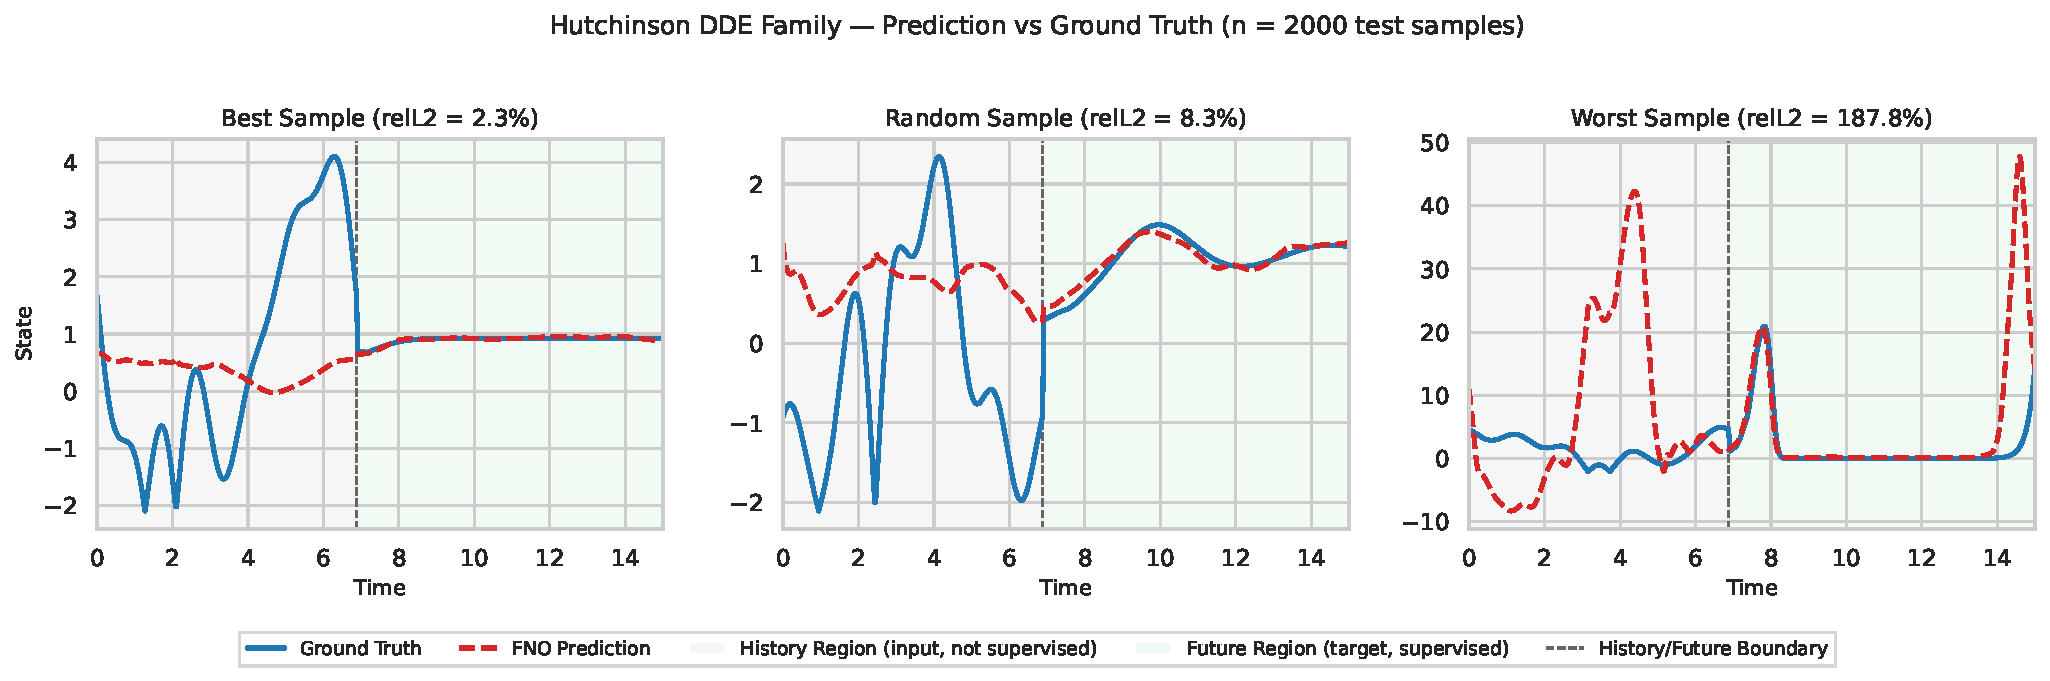
\includegraphics[width=\textwidth]{figures/hutch_hutch_with_regions.pdf}
  \caption{Hutchinson}
\end{subfigure}
\hfill
\begin{subfigure}[b]{0.48\textwidth}
  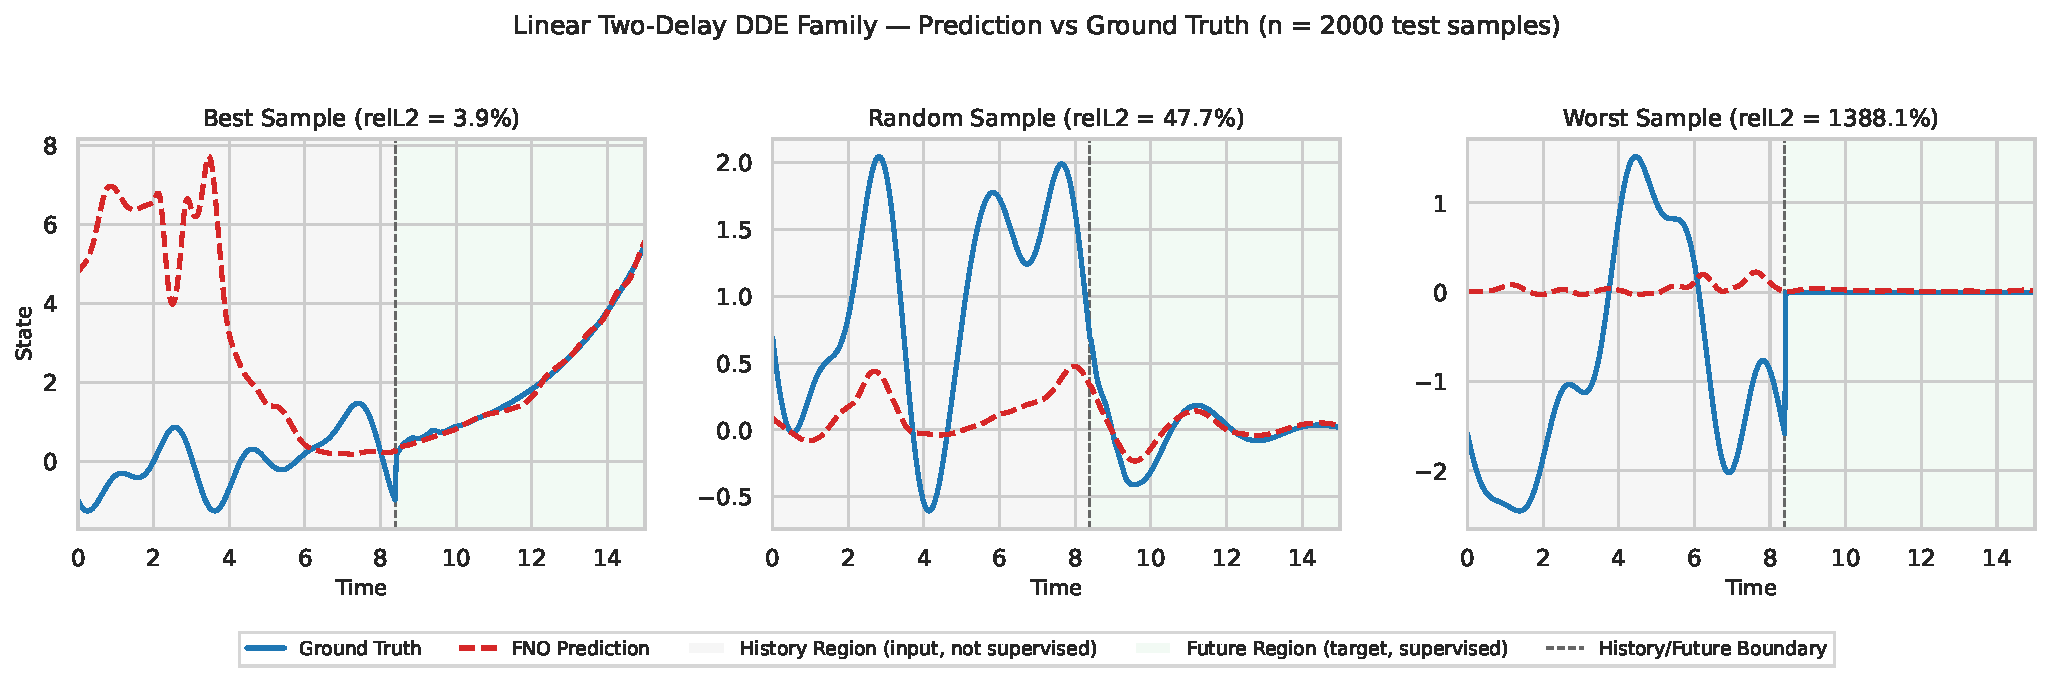
\includegraphics[width=\textwidth]{figures/linear2_linear2_with_regions.pdf}
  \caption{Linear2}
\end{subfigure}
\caption{Sample predictions with history (shaded) and future (white) regions.
Solid: ground truth; dashed: FNO prediction.}
\label{fig:predictions}
\end{figure}

% ------------------------------------------------------------------
\subsection{Out-of-Distribution Generalization}

Table~\ref{tab:ood-gaps} summarizes the OOD generalization gaps, defined as
the ratio of OOD median error to ID median error.  Larger gaps indicate worse
generalization.

\begin{table}[h]
\centering
\caption{Out-of-distribution generalization gaps (OOD median / ID median).
Higher values indicate worse generalization.}
\label{tab:ood-gaps}
\begin{tabular}{lccc}
\toprule
Family & OOD-delay & OOD-history & OOD-horizon \\
\midrule
Hutchinson  & 7.0$\times$ & 2.4$\times$ & 4.1$\times$ \\
Linear2     & 1.5$\times$ & 1.6$\times$ & 2.8$\times$ \\
Van der Pol & 2.6$\times$ & 4.0$\times$ & 4.3$\times$ \\
DistUniform & 5.1$\times$ & 11.3$\times$ & 2.4$\times$ \\
DistExp     & 4.2$\times$ & 3.9$\times$ & 1.5$\times$ \\
\bottomrule
\end{tabular}
\end{table}

\paragraph{OOD-delay.}
Extrapolation to unseen delay values produces the largest gaps for Hutchinson
(7.0$\times$) and DistUniform (5.1$\times$).  This is expected: the delay
$\tau$ directly controls the oscillation period in these families, so unseen
delays produce qualitatively different dynamics.  Linear2 shows a smaller gap
(1.5$\times$), likely because its difficulty is already high in-distribution.

\paragraph{OOD-history.}
Switching from Fourier-series histories (training) to cubic-spline histories
(test) reveals that models partially memorize the history function class.
DistUniform is most affected (11.3$\times$), suggesting the distributed-delay
averaging amplifies sensitivity to the smoothness structure of the input.

\paragraph{OOD-horizon.}
Extended prediction horizons ($T = 20$ vs.\ $T = 15$) generally produce moderate
gaps (1.5--4.3$\times$).  DistExp shows the smallest gap (1.5$\times$), as its
exponential kernel damps long-range dependencies.

Figure~\ref{fig:error-vs-time} shows the error-vs-time curve for Hutchinson across
all test splits, illustrating how errors accumulate over the prediction horizon and
diverge under distribution shift.

\begin{figure}[h]
\centering
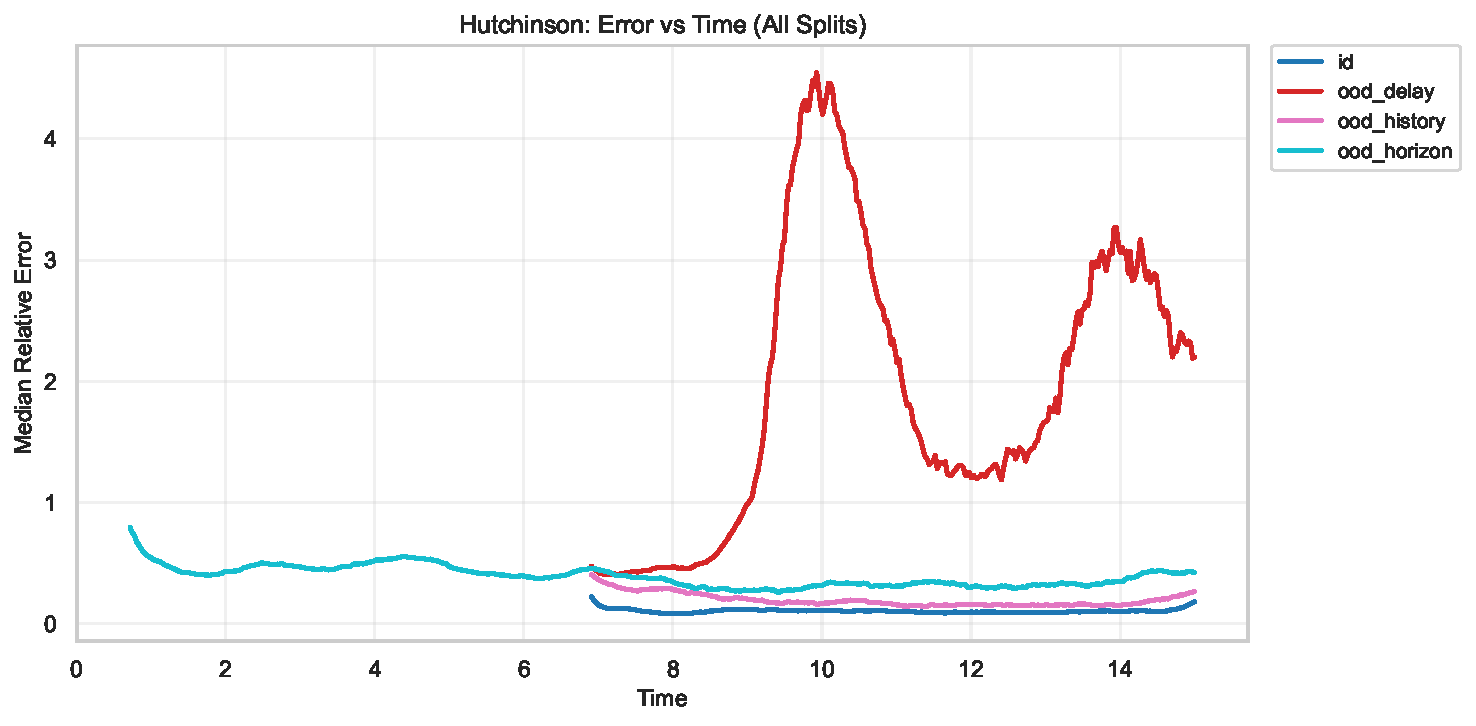
\includegraphics[width=0.65\textwidth]{figures/hutch_error_vs_time_all_splits.pdf}
\caption{Relative $L^2$ error vs.\ time for the Hutchinson family across ID and OOD
test splits.  Errors grow with prediction horizon and are amplified under distribution shift.}
\label{fig:error-vs-time}
\end{figure}

% ------------------------------------------------------------------
\subsection{Temporal Error Structure}

To understand how prediction quality degrades over time, we partition the
prediction horizon into three segments: Early $[0, 3.75]$, Mid $[3.75, 11.25]$,
and Late $[11.25, 15]$.  Table~\ref{tab:time-segments} reports the median
error in each segment.

\begin{table}[h]
\centering
\caption{Median relative $L^2$ error by time segment (ID test).}
\label{tab:time-segments}
\begin{tabular}{lccc}
\toprule
Family & Early & Mid & Late \\
\midrule
DistExp     & $<$0.001 & 0.034 & 0.022 \\
DistUniform & $<$0.001 & 0.047 & 0.049 \\
Hutchinson  & $<$0.001 & 0.063 & 0.102 \\
Van der Pol & $<$0.001 & 0.077 & 0.153 \\
Linear2     & $<$0.001 & 0.242 & 3.088 \\
\bottomrule
\end{tabular}
\end{table}

All families achieve near-zero error in the early segment, where the solution
is most constrained by the history function.  Errors grow monotonically for most
families, with Linear2 exhibiting a dramatic late-time blowup (mid: 0.24 $\to$
late: 3.09), indicating that the two interacting delays create compounding error
dynamics.  Notably, DistExp shows a slight \emph{decrease} from mid to late,
consistent with its exponential kernel damping long-range dynamics.

% ------------------------------------------------------------------
\subsection{Discussion}

Several patterns emerge from the baseline experiments:

\paragraph{Difficulty correlates with delay structure.}
Distributed delays (DistExp, DistUniform) are consistently easier than discrete
delays (Hutchinson, Van der Pol), which are in turn easier than multi-delay
systems (Linear2).  The integral averaging in distributed delays smooths the
operator's dependence on past states, producing a more regular input--output
mapping that is easier for the FNO to approximate.

\paragraph{The FNO's global receptive field is well-suited for delay dynamics.}
Unlike local methods (e.g., finite differences), the FNO's spectral convolution
captures long-range temporal dependencies in a single layer.  This is particularly
advantageous for DDEs, where the solution at time $t$ depends on values at $t - \tau$
that may be far away in the discretized sequence.  The 4.6--31.8$\times$ improvement
over the naive baseline confirms that the FNO learns meaningful delay structure.

\paragraph{OOD-history gaps reveal memorization of the history class.}
The large gaps under history distribution shift (up to 11.3$\times$ for DistUniform)
suggest that models partially memorize the smoothness properties of the Fourier-series
training histories rather than learning the underlying delay operator.  This motivates
training with diverse history function classes.

\paragraph{Multi-delay interactions remain challenging.}
Linear2's high ID error (0.612) and dramatic late-time blowup indicate that
the interaction of two delays $\tau_1$ and $\tau_2$ creates dynamics that are
fundamentally harder to approximate.  The FNO must implicitly learn the coupled
characteristic equation structure, which may require greater model capacity or
specialized architectures.

\subsection{Scope of the frozen baseline vs.\ extended benchmark}
\label{sec:scope-frozen-vs-phase-b}

The experiments reported in this section constitute the \emph{frozen
baseline}: a single FNO1d-Residual model ($\sim$93k parameters)
evaluated on five families across four OOD splits and one data scale.
Numerical results are reproducible from the manifest
\texttt{freeze\_manifest\_all5\_v2.json} and the tag
\texttt{baseline\_all5\_frozen\_v2}.

The extended benchmark (Phase B, specified in
\texttt{configs/sweep\_phase\_b.yaml}) broadens the evaluation along
three axes simultaneously.  Along the \emph{model} axis, the
11-model zoo from the experimental design document is ported and
smoke-tested: PlainMLP, MLP with cyclic-shift augmentation at two
budgets, FNO1d, DeepONet, MemNO, ANIE, LocalizedNO, LNO, MFNO, LEMO,
and LEMO$_{\sigma}$($\sigma = 0.9$).  Along the \emph{family} axis,
VdP and DistUniform are added and (pending data generation)
Mackey--Glass and Predator--Prey.  Along the \emph{split} axis,
continuous-$\tau$ evaluation is added for the three families where the
continuous-lag equivariance theorem is the most natural operational
story (DistExp, DistUniform, Hutchinson), and history-amplitude
evaluation for the three families most sensitive to initial-condition
magnitude (VdP, Mackey--Glass, Predator--Prey).  The full matrix is
$(7~\text{families}) \times (\text{applicable splits}) \times (12~\text{model entries}) \times (3~\text{seeds})
= 972~\text{runs}$, matching the plan's $\sim$700-run estimate after
dedup.  Results from this sweep will be reported in a revised version
of this section once the Mackey--Glass and Predator--Prey generators
and the continuous-$\tau$ off-grid data pipeline are available.
